\vspace*{-1mm}
The theoretical model for the transverse emittance growth caused by amplitude and phase noise in a CC was introduced in Chapter~\ref{Ch:CC_noise_theory}. In 2018, a dedicated experiment was conducted in the SPS to benchmark these models with experimental data and confirm the analytical predictions. Here, the objective is to provide an overview of the machine setup and the beam instrumentation used for the emittance growth studies with $\CC$s in the SPS.

The chapter is structured as follows: Section~\ref{sec:SPS_setup} describes the experimental machine configuration. Thereafter, Section~\ref{sec:CC_SPS_setup} elaborates on the installation and the operation of the CCs in the SPS. In Sections~\ref{sec:HT_info}-~\ref{sec:WallCurrentMonitor} the instruments used for the parameters of interest (see Chapter~\ref{Ch:CC_noise_theory}, Eq....) i.e. $\CC$ voltage, emittance and bunch length are discussed, including the post processing methods where it was performed by myself.

\section{Machine configuration}\label{sec:SPS_setup}
In view of the $\CC$s operation in HL-LHC where the beam will stay in the machine for sevral hours, special cycles were setup in the SPS for the emittance growth studies with $\CC$s. They are called "coast" bunched beam cycles and during them the bunches circulate in the machine at constant energy for long periods up to a few hours.

As the project of the CCs aims to the LHC were the beam stays in the machine for hours. Thus, for the emittance growth studies with CCs in the SPS special cycle was setup, which are called "coast" bunched beam cycles. This term 


a special machine configuration was set up called 'coast' beam cycles with bunched beam. 
Long time conservative


The available time for testing the CC noise induced emittance growth was very limited. Therefore, a number of thorogh preparatory have been performed in advance Ref[...]

One of the major concerns was the natural emittance growth observed in SPS in coast. The reason is not yet well understood. However, it was identified that is minimum for higher energies. Now the higher energy that the SPS can operate in coast is 270 GeV. Thus, the emittance growth experiemtns were performed at 270 GeV




A number of preparatory studies have been perforemd the years before 2018, in order to define the optimal machine configuration for the experimental study of the CC noise induced emittance growth.

- Energy
- chromaticity. Dependence of natural emittance growth to chromaticity. It was kept minimum. Measurements not available but we will consider small value ~ 1.
- To simplify the study the octupoles were switched OFF. For the model to apply we need a tune spread from amplitude detuning. THe octupoles were switched off as the resitudal non lineariteis Ref to micheles paper result to a sufficient tune spread of $10^-4$.

\section{Crab Cavities in the SPS}\label{sec:CC_SPS_setup}

For the SPS tests two prototype $\CC$s of the Double Quorter Wave (DQW) type were fabricated by CERN and were assembled into the same cryomodule which is shown in Fig.~\ref{fig:DQW_cryomodule}~\cite{Zanoni:2017}. The cryomodule was installed in the SPS-LSS6 zone, Fig.~\ref{fig:CC_SPS_LSS6}, and was placed on a mobile transfer table~\cite{Calaga:2649807}. The table moved with high precision and without breaking the vaccum the cryomodule in the beam line for the $\CC$ tests and out of it for the usual SPS operation. The main parameters for the $\CC$ experiments in SPS are shown in Table~\ref{tab:SPS_CC_main}


\begin{figure}[h]
   \centering         
   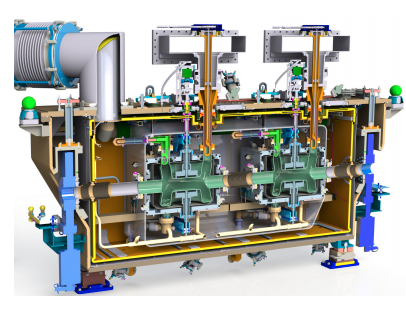
\includegraphics[width=0.8\textwidth]{images/Ch4/CC_cryomodule.png}
       \caption{Cut of the CC cryomodule~\cite{Zanoni:2017}.}
       \label{fig:DQW_cryomodule}
\end{figure}

\begin{figure}[h]
   \centering         
   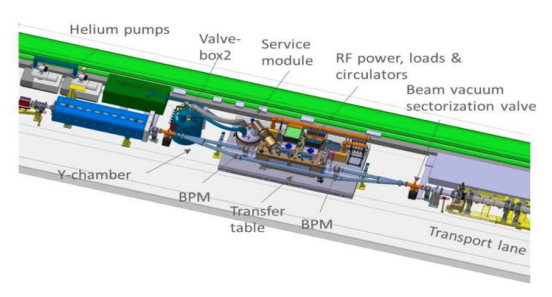
\includegraphics[width=0.8\textwidth]{images/Ch4/CC_location_SPS_LSS6.png}
       \caption{Installation of the cryomodule in the SPS-LSS6 zone~\cite{Calaga:2649807}.}
       \label{fig:CC_SPS_LSS6}
\end{figure}

\begin{table}[!hbt]
	\centering
   \caption{Main parameters for the emittance growth studies with CCs in SPS in 2018}
	\begin{tabu} to \textwidth { X[c,m] X[c,m] X[c,m] X[c,m] X[c,m] X[c,m] }
		&&&&& \\[-6mm]
		\toprule \toprule
		\multicolumn{2}{l}{\textbf{Parameters}} &
		\multicolumn{2}{c}{\textbf{Units}} &
		\multicolumn{2}{c}{\textbf{Values}} \\
		\bottomrule
      \multicolumn{2}{l}{$\symE$} & \multicolumn{2}{c}{[GeV]} & \multicolumn{2}{c}{26, 270} \\
      \multicolumn{2}{l}{Main RF frequency} & \multicolumn{2}{c}{[MHz]} & \multicolumn{2}{c}{200} \\
      \multicolumn{2}{l}{$\Qx$ / $\Qy$} & \multicolumn{2}{c}{[-]} & \multicolumn{2}{c}{26.13 / 26.18 } \\
      %\arrayrulecolor{black!30}\midrule
      \midrule
      \multicolumn{2}{l}{} & 	\multicolumn{2}{c}{} & \multicolumn{1}{c}{\textbf{CC1}} & \multicolumn{1}{c}{\textbf{CC2}} \\
      \midrule
      \multicolumn{2}{l}{crabbing plane} & \multicolumn{2}{c}{[-]} & \multicolumn{1}{c}{vertical} & \multicolumn{1}{c}{vertical} \\
      
      \multicolumn{2}{l}{s-location} & \multicolumn{2}{c}{[m]} & \multicolumn{1}{c}{6312.72} & \multicolumn{1}{c}{6313.32} \\

      \multicolumn{2}{l}{$\VCC$} & \multicolumn{2}{c}{[MV]} & \multicolumn{1}{c}{0} & \multicolumn{1}{c}{1} \\

      \multicolumn{2}{l}{$\fCC$} & \multicolumn{2}{c}{[MHz]} & \multicolumn{1}{c}{400} & \multicolumn{1}{c}{400} \\

      \multicolumn{2}{l}{$\beta_{x, CC}$ / $\beta_{y, CC}$} & \multicolumn{2}{c}{[m]} & \multicolumn{1}{c}{29.24 / 76.07} & \multicolumn{1}{c}{30.31 / 73.82} \\

      \multicolumn{2}{l}{$\alpha_{x, CC}$ / $\alpha_{y, CC}$} & \multicolumn{2}{c}{[m]} & \multicolumn{1}{c}{-0.88 / 1.9} & \multicolumn{1}{c}{-0.91 / 1.86} \\

      \multicolumn{2}{l}{$D_{x, CC}$ / $D_{y, CC}$} & \multicolumn{2}{c}{[m]} & \multicolumn{1}{c}{-0.48 / 0} & \multicolumn{1}{c}{-0.5 / 0} \\
      \arrayrulecolor{black}\bottomrule
 
	\end{tabu}
   \label{tab:SPS_CC_main}
\end{table}


%\large{\textbf{Operational considerations}}\\
\subsection{Operational considerations}

For the beam tests with the $\CC$s in the SPS the approach regarding the energy ramp and the adjustment of the phasing with the main RF system needed to be evaluated and they are briefly discussed here.


\normalsize{\textbf{Energy ramp}}\\
SPS recieves the beam at 26\,GeV. It was observed that if the ramp to higher energies was performed with the $\CC$ on, the beam was lost while crossing one of the vertical betatron sidebands due to resonant excitation~\cite{Rama_Paris_persentation}. Therefore, it was established that the acceleration has to be performed with the $\CC$ off and its voltage must be set up only after the energy of interest has been achieved. It should be noted here that this will be the approach also for the HL-LHC.

\normalsize{\textbf{Crab Cavity - main RF synchronisation}}\\
Another issue of concern was the fact that the $\CC$ operate at the fixed frequency of 400\,MHz while the SPS main RF system operates at 200\,MHz.
In order to make sure that the beam will experience the same effect from the $\CC$ each turn the SPS main RF has to be re-phased such as it becomes synchronous with the crabbing signal. For studies at the injection energy of 26\,GeV this synchronisation took place shortly after the injection. For studies at 270\,GeV, like the emittance growth measurements, the synchronisation took place at the end of the ramp shortly after the cavity was switched on~\cite{BE_seminar}.


\section{SPS Head-Tail monitor}\label{sec:HT_info}
The HT monitor was the main diagnostic device deployed for the callibration of the $\CC$ voltage. Additionally, it was used for the measurement and the physical illustration of the crabbing. This made it a very useful tool in the time of the experiments as it provided a direct validation of the effect of the $\CC$ kick on the beam. The HT monitor was originally designed for measuring chromaticity and transverse isntabilities. Therefore its use as a crabbing diagnostic should be explained here. The methods and procedures described in this section were developed at CERN and they are described here for the completness of the thesis.

 In the first part of this section some general information on the instrument along with example signals will be presented. Subsequently, the post processing of the HT signal in the presence of the $\CC$s. Last, the callibration of the $\CC$ voltage from the HT data is described. The experiemental data presented in this section were acquired at the SPS injection energy of 26\,GeV with only one $\CC$, $\CC$1, at $\phiCC=0$ for simplicity. That energy option was chosen as the effect of $\CC$ kick on the beam is stronger and thus more visible than in higher energies.



\normalsize{\textbf{General information}}\\
\begin{figure}[h]
   \centering         
   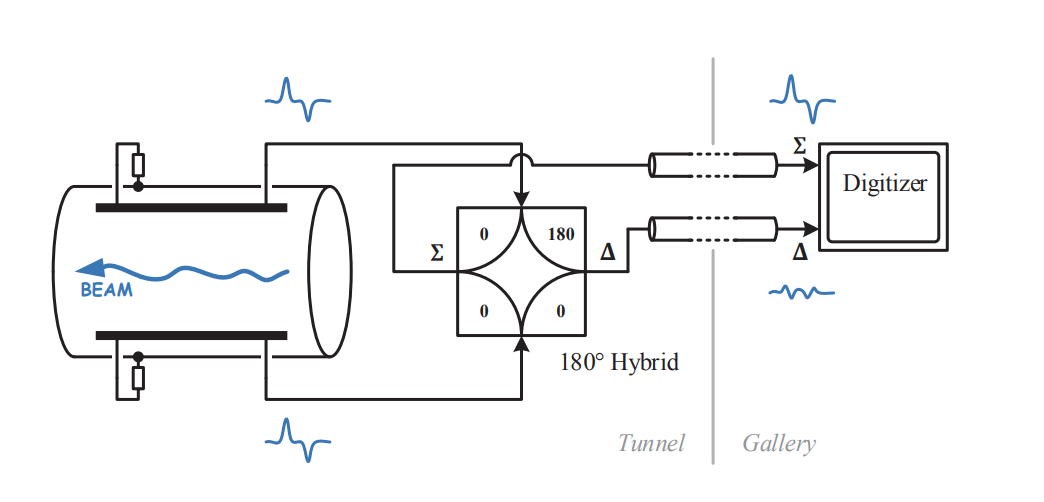
\includegraphics[width=0.7\textwidth]{images/Ch4/SPS_HT_monitor_diagram_modified.png}
       \caption{Diagram of the SPS HT monitor~\cite{Levens:2313358}.}
       \label{fig:SPS_HT_diagram}
\end{figure}
The HT monitor is a high bandwidth version of a standard beam position monitor but it can measure the transverse offset within the bunch. This makes it ideal for the measurement of the intra-bunch offset caused from the $\CC$ kick. Its reading consists of the sum $\Sigma$ and the  difference $\Delta$ of the electrode signals of a straight stripline coupler (Fig.~\ref{fig:SPS_HT_diagram})~\cite{Jones:987561, Levens:2313358} over a defined acquisition period. The $\Sigma$ signal is the longitudinal line density while the $\Delta$ signal corresponds to the intra-bunch offset. 

The raw signals from the HT monitor require a specific post processing procedure, which is described in Ref.~\cite{Levens:2313358}, in order to give useful information. Figure~\ref{fig:HT_example_signals} shows some example signals obtained from the HT monitor after the basic post procesing is applied. Moreover, Fig.~\ref{fig:HT_example_signals_2D} shows a 2D representation of the HT monitor reading. It is worth noting here that in the specific example a clear periodic oscillation of the vertical intra-bunch offset (vertical $\Delta$) signal is observed. This is a result of the main RF system not being synchronous with the  $\CC$  frequency. 

% COMMENT: The Ref.~\cite{Levens:2313358} refers to the LHC HT monitor but the same applies for SPS as it is the same device.


\begin{figure}[!h]
   \centering         
   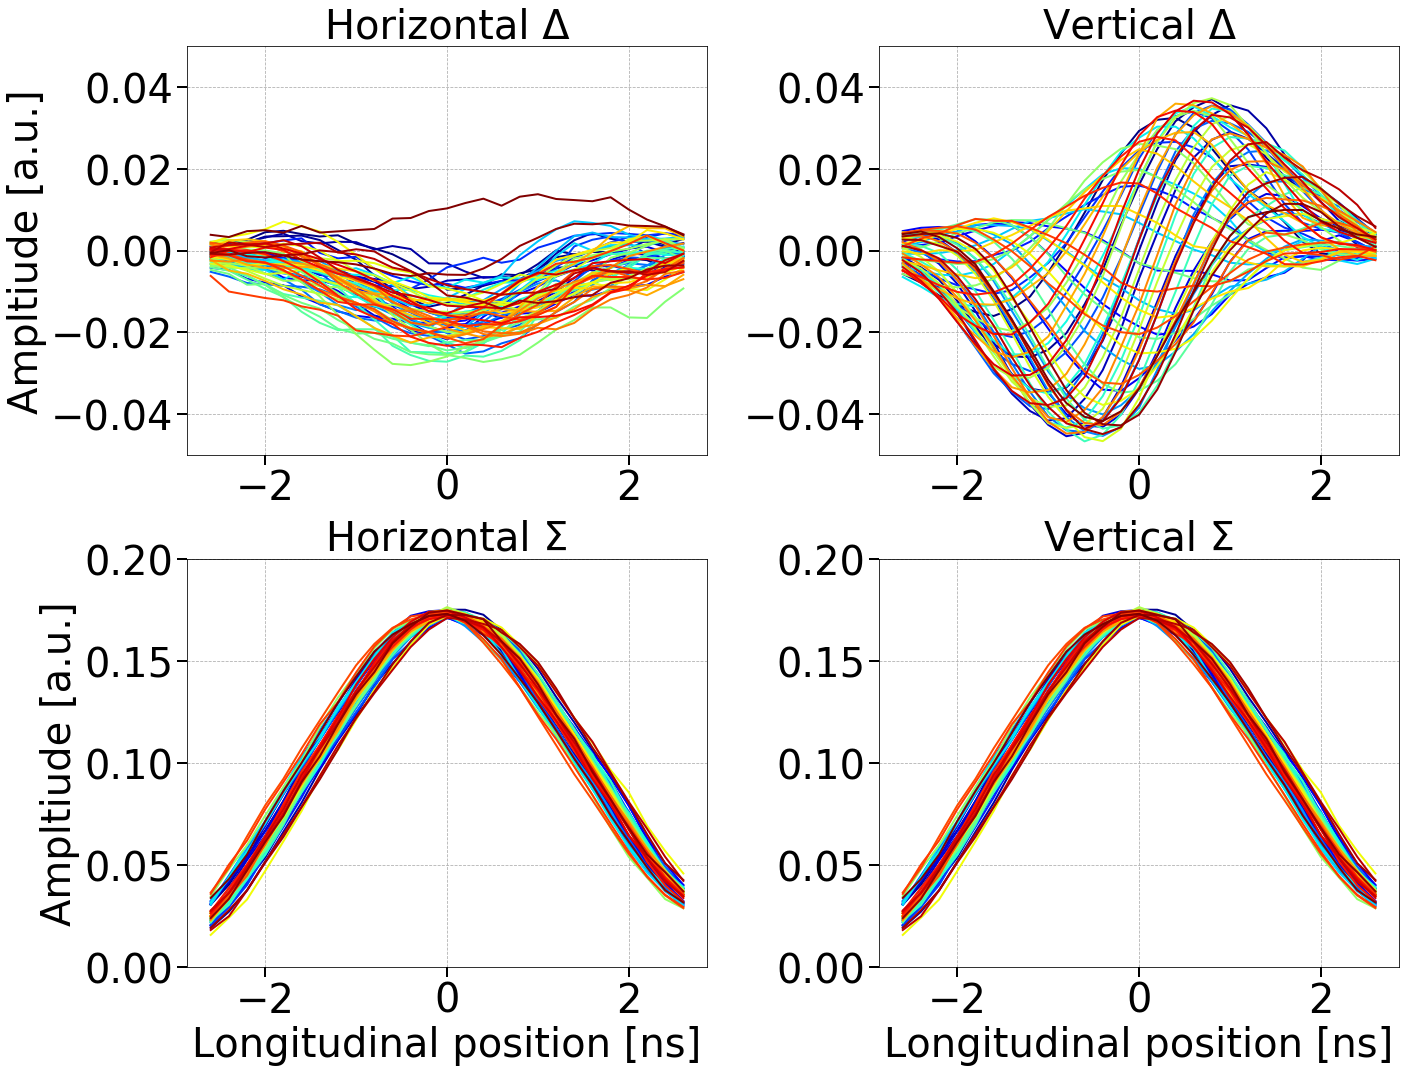
\includegraphics[width=0.8\textwidth]{images/Ch4/HT_1D__20180530_135105exampleAcq_4thesis_turnsStart0_Stop6000_step100_new.png}
       \caption{Example $\Delta$ and $\Sigma$ signals from the HT monitor with respect to the longitudinal position within the bunch over several SPS revolutions, after the basic post processing (Ref.~\cite{Levens:2313358}) but before the baseline correction. The different colors indicate the signals from different turns.}
       \label{fig:HT_example_signals}
\end{figure}

\begin{figure}[!h]
   \centering         
   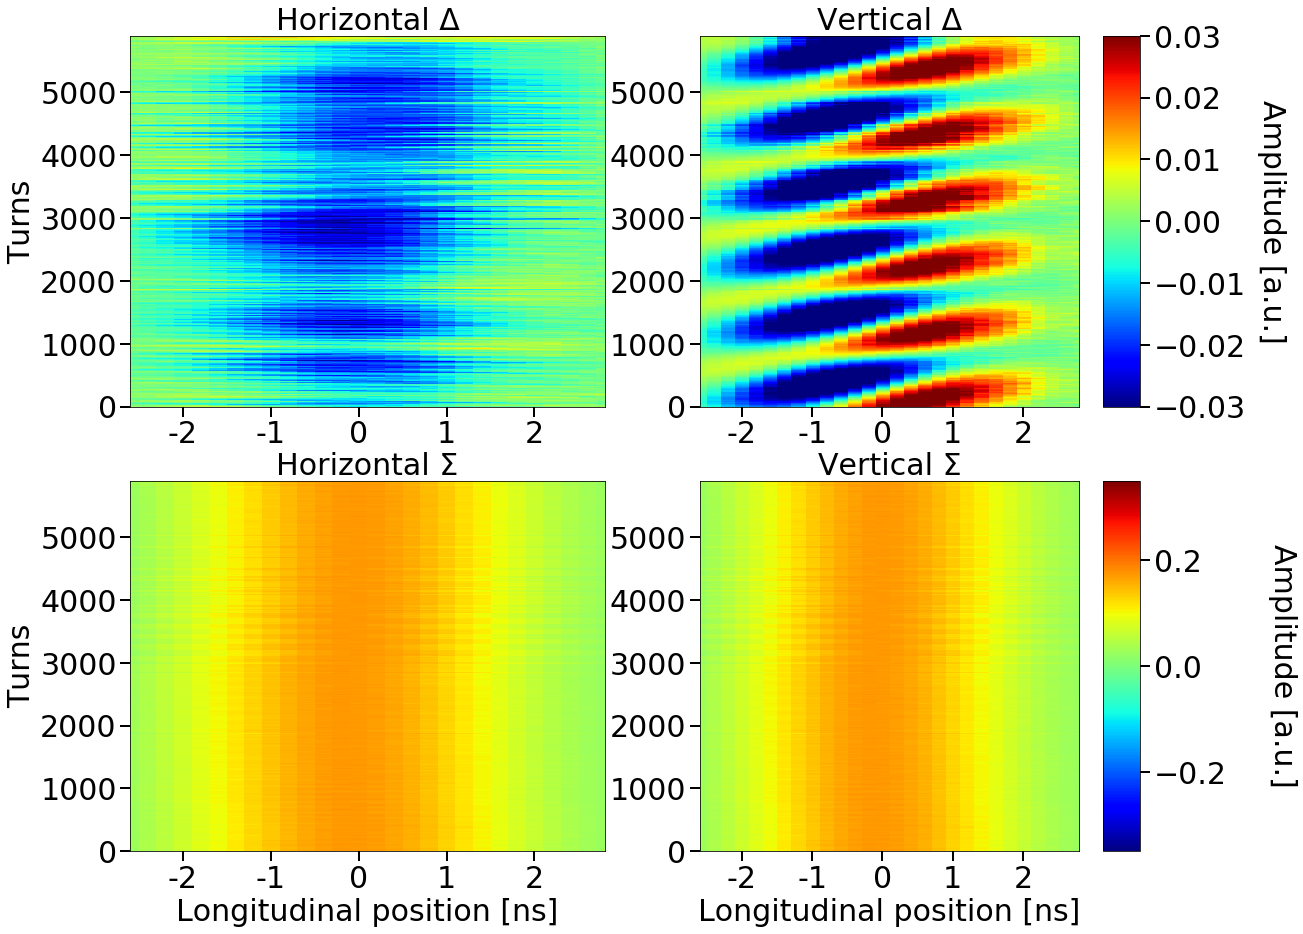
\includegraphics[width=0.9\textwidth]{images/Ch4/HT_2D__20180530_135105_colorbar_new_version.png}
       \caption{2D representation of example $\Delta$ and $\Sigma$ signals with respect to the longitudinal position within the bunch obtained from the HT monitor over several SPS revolutions.}
       \label{fig:HT_example_signals_2D}
\end{figure}


\subsection{Post processing in the presence of Crab Cavities}\label{subsec:HT_post_process_CC}
To obtain useful information from the HT monitor signal in the presence of the $\CC$s there are a few steps that differ from the standard post processing procedure and they are desribed below.

\normalsize{\textbf{Heat-Tail monitor baseline correction}}\\
One issue of concern is the correction of the $\Delta$ signal  baseline due to orbit offsets and non-linearities of the instrument~\cite{Levens:2313358}. During the normal post processing, the correction is achieved by computing the mean of the $\Delta$ signals over all turns and then subtracting this static offset from the signal of each turn. However, in the SPS tests, where the $\CC$s are well synchronised with the main RF system (Section~\ref{sec:CC_SPS_setup}), the crabbing signal is also a static intra-bunch position offset and thus would also be removed with the usual method.

Therefore, for the $\CC$ experiments a reference measurement had first to be made with the $\CC$ unsynchronised. The mean of the $\Delta$ signal over this reference period was the baseline which then was subtracted from the $\Delta$ signals acquired after the synchronisation (Fig~\ref{fig:HT_baseline_correction}). The datasets before and after synchronisation are easily distinguishable in the 2D HT monitor reading as displayed in Fig.~\ref{fig:HT_baseline_correction_measurements_2D}


\begin{figure}[!h]
   \centering         
   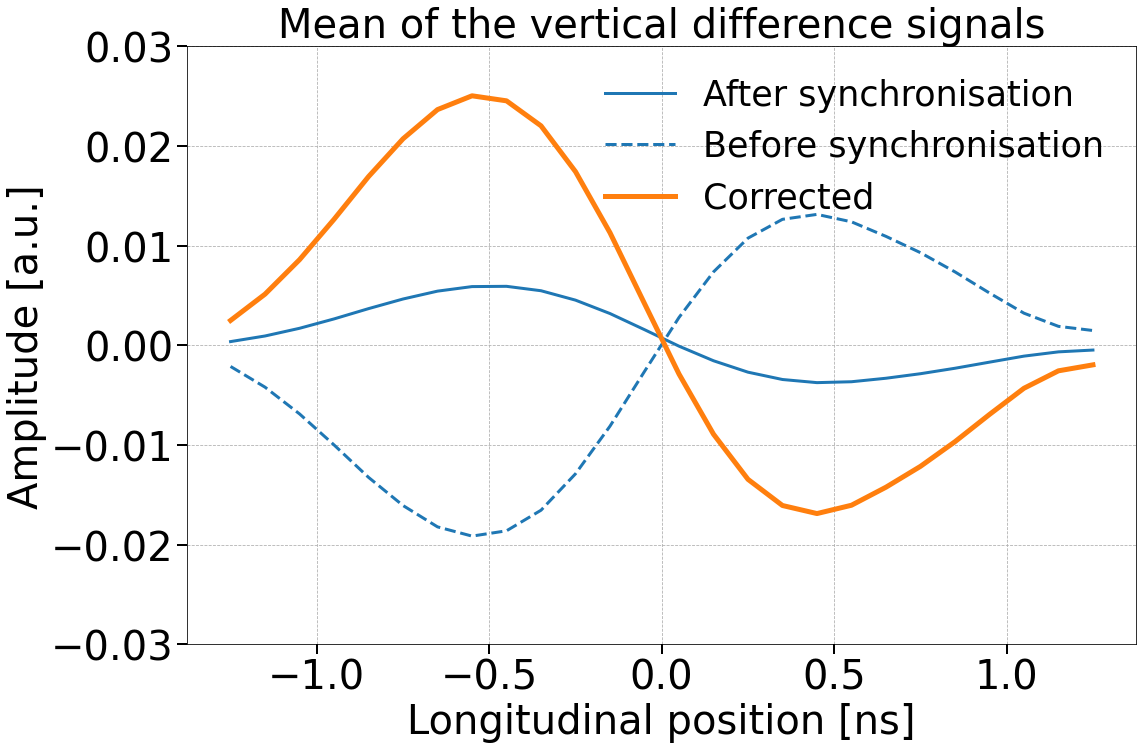
\includegraphics[width=0.65\textwidth]{images/Ch4/HT_measures_vs_reference_vs_corrected__20180530_135105_baseline_correction_new_version.png}
       \caption{HT monitor baseline correction for the SPS CC tests.}
       \label{fig:HT_baseline_correction}
\end{figure}

\begin{figure}[!h]
   \centering         
   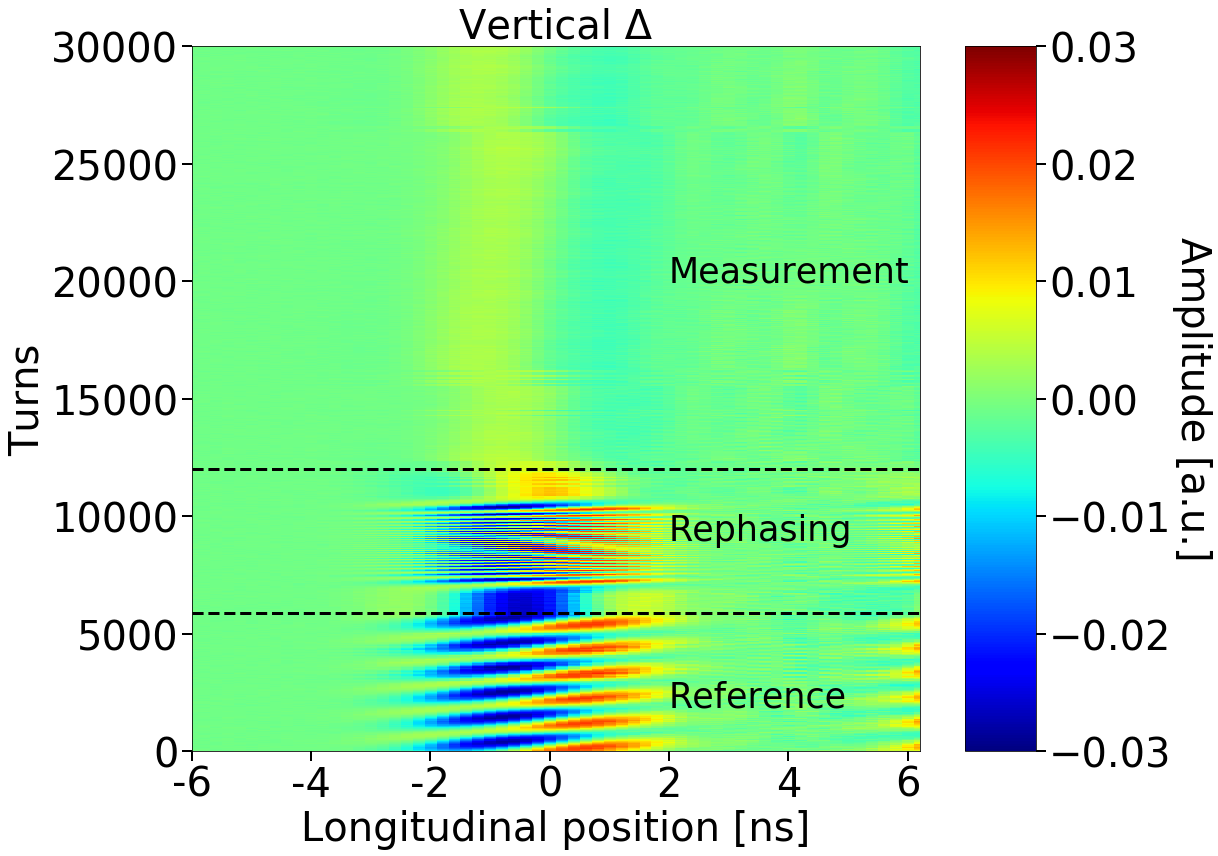
\includegraphics[width=0.7\textwidth]{images/Ch4/HT_2D__20180530_135105_before_after_sunchronisation_new_version.png}
       \caption{HT acquistions before and after the sunchronisation of the SPS main RF with the CC.}
       \label{fig:HT_baseline_correction_measurements_2D}
\end{figure}


\normalsize{\textbf{Headtail monitor callibration}}\\
The last step, to make the HT acquisitions meaningful is to convert the measured intra bunch offset, $\langle \Delta \rangle$, from arbitrary units to mm. The scaling is achieved by division with the $\langle \Sigma \rangle$ signal and with a normalisation factor which is provided by the calibration of the HT monitor~\cite{PhysRevAccelBeams.22.112803}. The normalisation factor for the SPS was measured at 0.1052 in 2018~\cite{HT_calibration_2018}. Figure~\ref{fig:HT_baseline_correction_crabbing_mm} shows the intra bunch offset from the CC kick in mm and after the baseline correction. 


\begin{figure}[!h]
   \centering         
   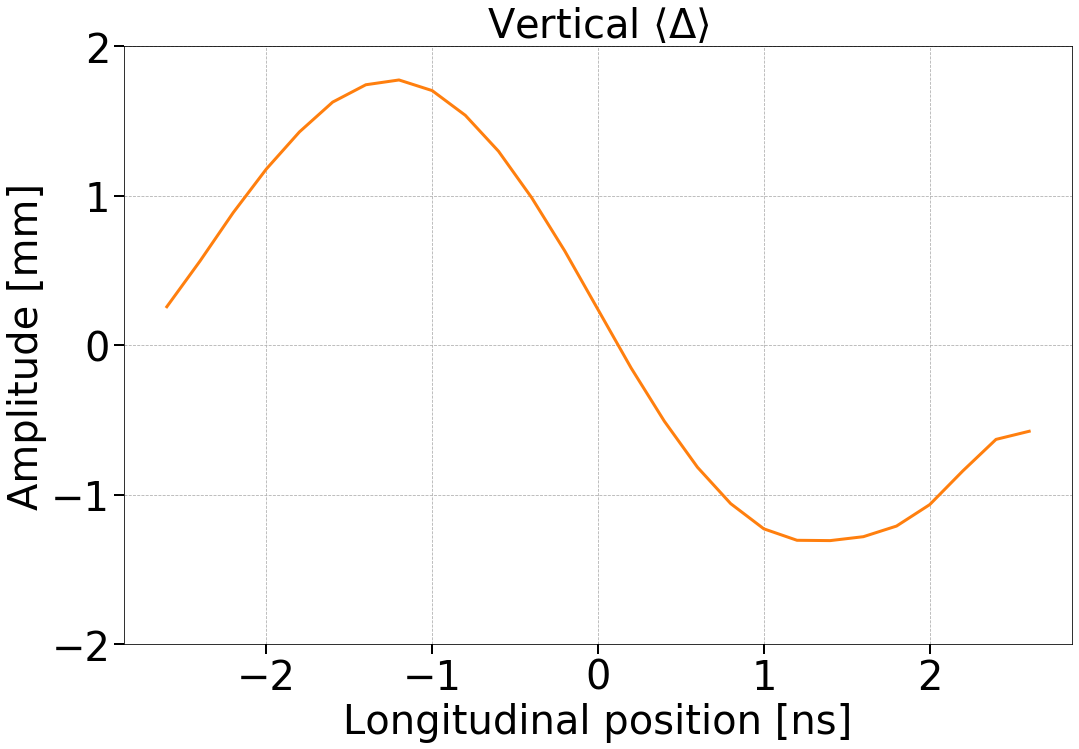
\includegraphics[width=0.65\textwidth]{images/Ch4/HT_corrected__20180530_135105_baseline_correction_new_version.png}
       \caption{Intra-bunch offset from the CC kick expressed in mm after the removal of the baseline.}
       \label{fig:HT_baseline_correction_crabbing_mm}
\end{figure}




 \subsection{Crab Cavity voltage calibration}\label{sec:Vcc_calibration}
 This section discusses the beam based measurement of the $\CC$ voltage from the HT monitor signal. The calibration was performed by calculating the kick required to reconstruct the measured intra-bunch offset using Eq.~\eqref{eq:CC_orbit_shift_Chao}. Equation~\eqref{eq:CC_orbit_shift_Chao}, which is obtained from Chaos' Eq.\,(1) from chapter 4.7.1 in Ref.~\cite{Chao:1490001}, gives the vertical orbit shift (in meters) from the $\CC$ kick, $\theta$, at the HT monitor location as follows:


\begin{equation}\label{eq:CC_orbit_shift_Chao}
   \Delta y_{,HT} = \frac{\sqrt{\beta_{y, HT}}}{2 \sin(\pi \Qy)} \theta \sqrt{\beta_{y, CC}} \cos(\pi \Qy - \mid \psi_{y, HT} - \psi_{y, CC} \mid),
\end{equation}

where $\beta_y$ is the beta function, $\Qy$ is the tune, and $\psiy$ is the phase advance in tune units. The same applies for the horizontal plane. The indeces HT and CC indicate the optic parameters at the location of the HT monitor and CC respectively.

The deflection from the $\CC$ is written as $\theta = - \frac{q V(t)}{\symE}$, where q is the charge of the particle, $\symE$ the beam energy and $V_{CC}(t) = \VCC \sin(2 \pi \fCC t + \phiCC) $ is the voltage that a particle experiences while passing through the $\CC$. Computing the maximum of $V_{CC}(t)$ gives the cavity voltage, $\VCC$. 

\begin{figure}[!h]
\centering         
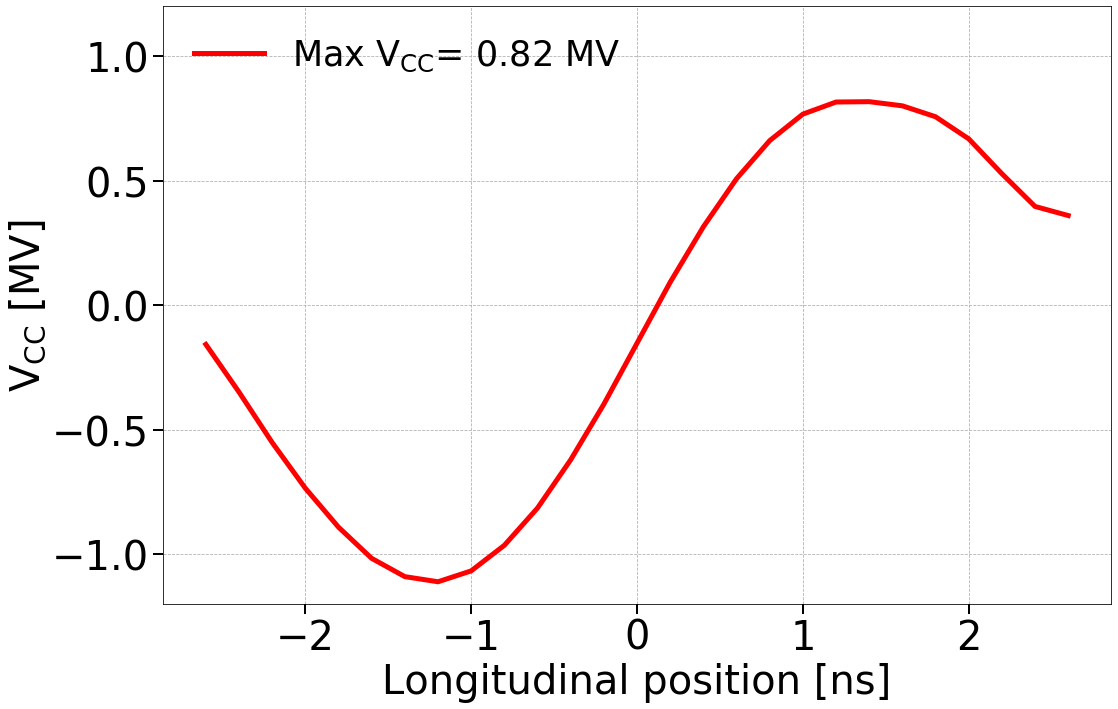
\includegraphics[width=0.65\textwidth]{images/Ch4/HT_VCC_callibration_20180530_135105.png}
    \caption{CC voltage calibration from the HT monitor.}
    \label{fig:VCC_from_HT_monitor_measurement}
\end{figure}

It should be noted here, that the measured intra-bunch offset, $\Delta y_{, HT}$, is inserted in Eq.~\eqref{eq:CC_orbit_shift_Chao} after removing the baseline and converting it in mm as discussed in Section~\ref{subsec:HT_post_process_CC}. Figure~\ref{fig:VCC_from_HT_monitor_measurement} illustrates the cavity voltage computed from the HT signals shown already in this section. The corresponding beam and optic parameters are listed in Table~\ref{tab:SPS_HT_CC}



\begin{table}[!hbt]
	\centering
   \caption{Parameters for computing the CC voltage from the example HT monitor measurements discussed in this chapter}
	\begin{tabu} to \textwidth { X[c,m] X[c,m] X[c,m] X[c,m] X[c,m] X[c,m] }
		&&&&& \\[-6mm]
		\toprule \toprule
		\multicolumn{2}{l}{\textbf{Parameters}} &
		\multicolumn{2}{c}{\textbf{Units}} &
		\multicolumn{2}{c}{\textbf{Values}} \\
		\bottomrule
      \multicolumn{2}{l}{$\beta_{y, HT}$ / $\beta_{y, CC1}$}& \multicolumn{2}{c}{[m]} & \multicolumn{2}{c}{49.19 / 76.07} \\
      \multicolumn{2}{l}{$\psi_{y, HT}$ / $\psi_{y, CC1}$} & \multicolumn{2}{c}{[-]} & \multicolumn{2}{c}{15.68 / 23.9} \\
      \multicolumn{2}{l}{$\Qy$} & \multicolumn{2}{c}{[-]} & \multicolumn{2}{c}{26.13} \\
      \multicolumn{2}{l}{$\symE$} & \multicolumn{2}{c}{[GeV]} & \multicolumn{2}{c}{26} \\
      \bottomrule
	\end{tabu}
   \label{tab:SPS_HT_CC}
\end{table}

\normalsize{\textbf{Reconstruction of crabbing}}\\
The reconstruction of the crabbing from the HT monitor measurements and the physical illustration of it are paresented here. This technique was developed at CERN in 2018 and it was extensivley used throught the experimental campaign with $\CC$s as alongside the calibrated voltage it gives a straightforward estimation of the applied $\CC$ kick, as illustrated in Fig.~\ref{fig:crabbing_reconstruction_HT_monitor}. \\ \\
To obtain this physical illustration of the effect of the CC kick on the beam one needs to modualte the measured longitudinal profile, $\langle \Sigma \rangle$, with the measured intra-bunch offset (e.g. Fig.~\ref{fig:HT_baseline_correction_crabbing_mm}). For the transverse plane a gaussian distribution is considered with $\sigma$ obtained from the wire scanner (addressed in more details in the following section). The color code is normalised to the maximum intensity within the bunch.

\begin{figure}[!h]
   \centering         
   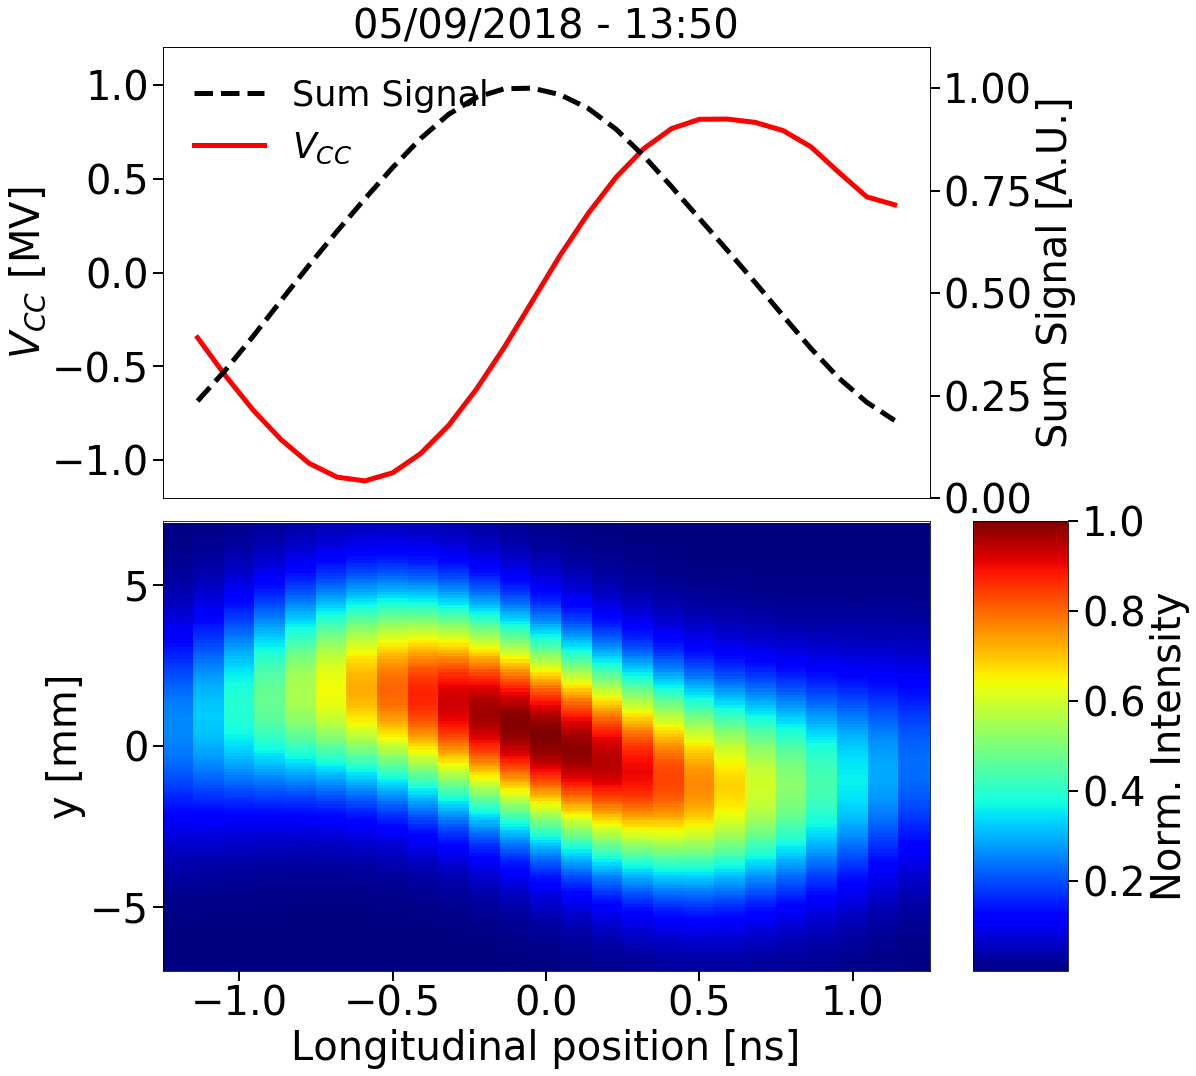
\includegraphics[width=0.7\textwidth]{images/Ch4/HT_crabVoltage__20180530_135105_crabbing_only.png}
       \caption{Illustration of the crabbing from the HT monitor signal.}
       \label{fig:crabbing_reconstruction_HT_monitor}
\end{figure}
   



\section{SPS Wire Scanners}

The SPS is equpped with beam wire scanners (WS) to measure the transverse beam emittance. The SPS WS system is described in detail in Ref.~\cite{BOSSER1985475, Berrig:1972478}. For the SPS tests, the emittance was measured with rotational WS both for the horizontal and vertical plane (BWS.51995.H and BWS.41677.V respectively).

The working principle is shown in Fig.~\ref{fig:SPS_WS_ROT}. A thin wire rapidly moves across the proton beam and a shower of secondary particles is generated. Their signal is then detected by a system of scintillator/photomultiplier (PM) outside of the beam pipe. By measuring the wire position and the PM current at it over multiple turns the transverse beam profile is reconstructed. An example of a vertical profile is shown in Fig.~\ref{fig:WS_example_V_profile} (left).


\begin{figure}[!h]
   \centering         
   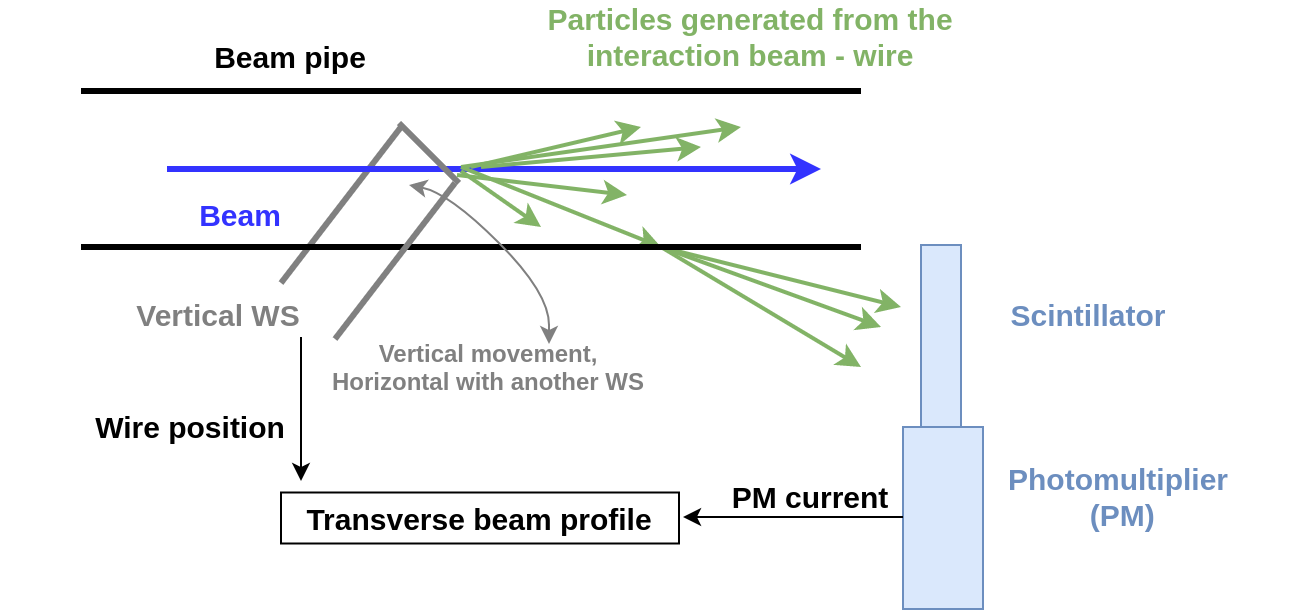
\includegraphics[width=0.8\textwidth]{images/Ch4/Wire_scanner.png}
       \caption{Sketch of the SPS rotational wire scanners~\cite{Berrig:1972478}}
       \label{fig:SPS_WS_ROT}
\end{figure}


\normalsize{\textbf{Fitting of transverse profiles}}\\
To obtain the beam size, $\sigma$, the transvserse profiles from each scan are fitted with a four parameter Gauss function:

\begin{equation}\label{eq:4p_gauss}
   f(x) = k + A e^{-\frac{(x-\mu)^2}{2 \sigma^2}},
\end{equation}

where $k$ is the signal offset of the PM, $A$ is the signal amplitude, $\mu$ is the mean of the Gaussian distribution and $\sigma$ its standard deviation. The uncertainty of the measured beam size, $\Delta \sigma$, is defined as the one standard deviation error on $\sigma$ which is computed from the square root of the diagonal elements of the covariant matrix.
%https://docs.scipy.org/doc/scipy/reference/generated/scipy.optimize.curve_fit.html

\begin{figure}[!h]
   \centering
   \begin{subfigure}{.5\textwidth}
     \centering
     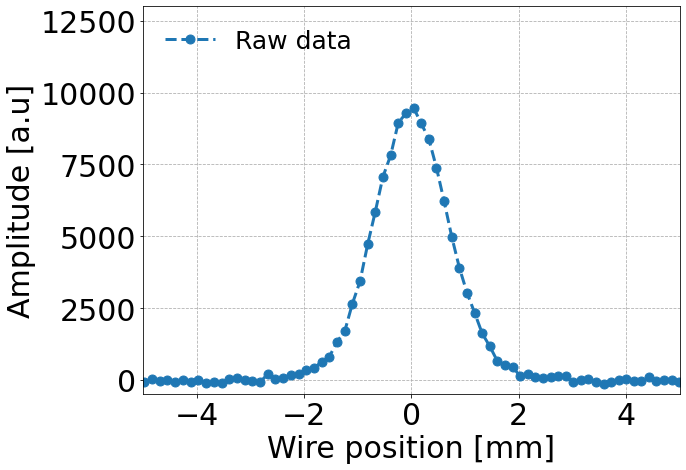
\includegraphics[width=1.0\linewidth]{images/Ch4/SPS.BWS.41677.V_ROT_2018-09-05 15_45_01.33500_raw.png}
   \end{subfigure}%
   \begin{subfigure}{.5\textwidth}
     \centering
     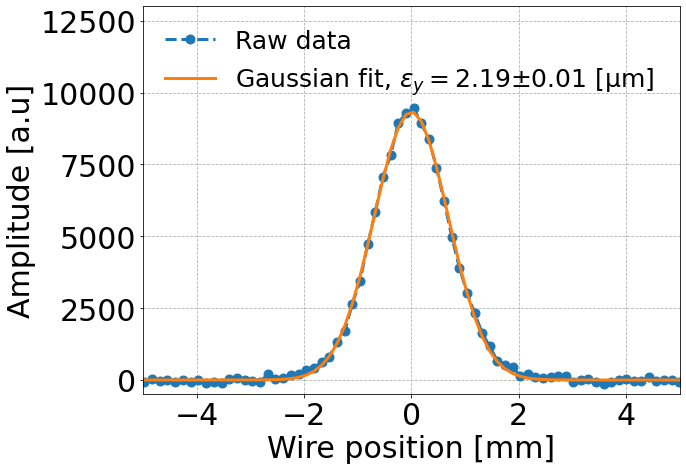
\includegraphics[width=1.0\linewidth]{images/Ch4/SPS.BWS.41677.V_ROT_2018-09-05 15_45_01.33500_raw_and_fit.png}
   \end{subfigure}
   \caption{ Vertical beam profile obtained from the BWS.41677.V instrument. The measuremed data points (light blue) are fitted with a four parameter Gaussian (orange) to obtain the beam size. The calculated emittance is also shown.}
   \label{fig:WS_example_V_profile}
\end{figure}

The general formula for computing the normalised beam emittance from the beam size, $\sigma$ is described in Eq.~\eqref{eq:emit_from_beam_size}. However, in the 2018 SPS operational configuration, the dispersion was small in the WSs location and thus its contribution to the beam size was considered to be negligible \footnote{The dispersion at BWS.51995.H location in 2018 was $D_x$= -15\,mm. At 270\,GeV, $\delta$ is of the order of $\mathrm{10^{-4}}$. Thus, from Eq.~\eqref{eq:emit_from_beam_size} the horizontal normalised emittance from the dispersion is foreseen at the order of $\mathrm{10^{-11}}$. Comparing to the observed beam size during the CC tests of a few microns the dispersion is negligible}. In that case, the normalised emittance can be calculated for both transverse planes simply from the beam size ($\sigma$), the beta function at the WS location ($\beta_{WS}$), and the relativistic parameters ($\betarel, \gammarel$) as follows:

\begin{equation}\label{eq:emittance_from_WS}
   \centering
   \epsilon = \frac{\sigma^2}{\beta_{WS}} \betarel \gammarel
\end{equation}

The beta functions were 81.5\,m and 62.96\,m at the locations of the horizontal and vertical WS respectively.

Considering that the relativistic parameters and the beta fucntion are free of error, the uncertainty of the computed emittance, $\Delta \epsilon$, at a dispersion free region, depends only on the uncertainty of the measured beam size, $\Delta \sigma$, as:

\begin{equation}\label{eq:emittance_from_WS_uncertainty}
   \centering
   \frac{\Delta \epsilon}{\epsilon} = \sqrt{\left(2\frac{\Delta \sigma}{\sigma} \right)^2} = 2\frac{\Delta \sigma}{\sigma},
\end{equation}


\normalsize{\textbf{Further considerations}}\\
It is worth noting here, that during each measurement with the WS the beam profile is actually acquired twice as the wire crosses the beam at the forward direction (IN scan) and then backwords (OUT scan). For the 2018 measurements the emittance values obtained from IN and OUT scans, $\epsilon_{IN} \pm \Delta \epsilon_{IN}$ and $\epsilon_{OUT} \pm \Delta \epsilon_{OUT}$ ,were found to be very similar (add order of difference). In this thesis, the average emittance from the two scans, $\epsilon_{avg} = \langle \epsilon_{IN}, \epsilon_{OUT}\rangle$ , will be used. The uncertainty on the averaged emittance, $\Delta \epsilon_{avg}$, is computed as:

\begin{equation}\label{eq:avg+emittance_from_WS_uncertainty}
   \Delta \epsilon_{avg} = \sqrt{\Delta \epsilon_1 ^2 + \Delta \epsilon_2 ^2},
\end{equation}
where $\Delta \epsilon_1$ is the standard deviation of the $\epsilon_{IN}$ and $\epsilon_{OUT}$ and $\Delta \epsilon_2=\sqrt{\langle \Delta \epsilon_{IN}, \Delta \epsilon_{OUT}\rangle}$.


Finally, some emittance increase is expected during each wire scan, due to Coulomb multiple scattering. This effect has been extensivley studied in Ref.~\cite{Roncarolo:1481835}. For the rotational SPS WS and the energy of 270\,GeV, at which the $\CC$ experiments were performed the expected emittance growth from the WS is expected to be small. However, a conservative number of scans were carried, $\sim$ 20 scans per bunch and per plane during $\sim$ 1 hour, in order to minimise the contribution from this effect.

\section{ABWLM}\label{sec:ABWLM}

\section{Wall current monitor}\label{sec:WallCurrentMonitor}

\section{Conclusions}

Post processing steps for the ones I have performed the analysis. The others just menitoned.
